% Jarvis: A Deterministic-First Local Voice Assistant
% Build: pdflatex jarvis.tex  (twice, for references)
\documentclass[10pt,twocolumn]{article}

\usepackage[margin=0.75in]{geometry}
\usepackage{times}
\usepackage{amsmath,amssymb}
\usepackage{graphicx}
\usepackage{booktabs}
\usepackage{multirow}
\usepackage{url}
\usepackage[hidelinks]{hyperref}
\usepackage{tikz}
\usetikzlibrary{arrows.meta,positioning,shapes.geometric,calc,fit,backgrounds}
\usepackage{listings}
\usepackage{xcolor}
\usepackage{caption}

\definecolor{det}{RGB}{31,119,180}
\definecolor{mod}{RGB}{214,39,40}
\definecolor{ver}{RGB}{44,160,44}
\definecolor{bg}{RGB}{245,245,245}

\lstset{
  basicstyle=\ttfamily\scriptsize,
  backgroundcolor=\color{bg},
  frame=single,
  breaklines=true,
  columns=fullflexible,
  showstringspaces=false,
  keywordstyle=\color{det}\bfseries,
}

\newcommand{\code}[1]{\texttt{\small #1}}

\title{\vspace{-1.5em}\textbf{Jarvis: A Deterministic-First Architecture for\\
Local Voice Assistants with a Small Language Model}}

\author{
  Ashutosh Kumar Singh\\
  \small Independent Research\\
  \small \texttt{ashutoshkumarsingh0x@gmail.com}
}

\date{July 2026}

\begin{document}
\maketitle

\begin{abstract}
\noindent
We describe Jarvis, an always-on local voice assistant built on a 4-billion-parameter
language model (\code{gemma3:4b}) running entirely on consumer hardware. The central
design claim is that for a large class of real user queries, the language model should
not produce the answer at all. Instead, a deterministic intent router dispatches to
handlers that read live ground truth --- on-chain RPC endpoints, financial APIs,
government and security feeds, and operating-system telemetry --- and the model is
reserved for open-ended synthesis.

We evaluate this claim with a 1000-prompt routing harness generated from catalogues
already present in the system, and measure that \textbf{95.3\%} of a realistic finance
and blockchain prompt set is answerable without invoking the model, at a routing cost of
\textbf{102\,$\mu$s} per prompt versus a measured \textbf{26.7\,s} mean per model turn.
Routing accuracy is \textbf{99.4\%} (994/1000). The harness surfaced four live
misrouting defects that months of hand-written tests had not.

Beyond routing we describe five further subsystems developed under the same discipline:
a hybrid BM25 + dense retrieval layer with an inverted index (230--320$\times$ faster
than the naive implementation, rankings bit-identical); a typed, revisable project
memory with per-type retention; an evidence-gated promotion mechanism in which repeated
observations sharing a dependency count once, not many times; an implicit-feedback
analyser that collapses 22 raw failure signals from a real 229-turn interaction log into
18 distinct user struggles; and a source planner whose per-source latencies are learned
by exponentially weighted moving average rather than hardcoded.

We report a measurement that reframes the parallelism problem: fetching seven live feeds
sequentially cost 6560\,ms versus 1652\,ms in parallel (3.97$\times$), but the parallel
total landed within 2\,ms of the \emph{slowest single source}. Selecting only the two
sources a query needs cost 24\,ms --- roughly 69$\times$ better, and an order of
magnitude beyond what fan-out alone can reach. We further report that this same
benchmark, re-run on unchanged code two days later, returned 4248\,ms / 938\,ms, a 36\%
shift attributable entirely to network conditions.

The system comprises 34 test suites and 1373 assertions. We are explicit throughout
about what is measured, what is asserted, and what remains unbuilt.
\end{abstract}

%------------------------------------------------------------------
\section{Introduction}

Voice assistants built on large language models typically place the model on the
critical path for every query. The model receives a transcript, decides what to do, and
generates the reply. When the model is a frontier system behind an API, this is
defensible. When the model is a 4-billion-parameter open-weight model running locally on
a laptop, it is not.

Jarvis is a local-first desktop assistant: Electron main process, Three.js shader
visualiser, always-on speech capture through \code{faster-whisper}, Windows SAPI
text-to-speech, and \code{gemma3:4b} served by Ollama. No cloud inference is used. The
constraint that follows from this is severe and quantifiable: a single model turn costs
a measured mean of 26.7\,s (p50 30.4\,s, p95 46.0\,s at concurrency 8). A voice
assistant that waits 30 seconds before speaking is not a voice assistant.

The architectural response is to invert the usual arrangement. Rather than asking how to
make a small model behave like a large one, we ask how often the model is needed at all.

\subsection{Contributions}

\begin{enumerate}\itemsep2pt
\item \textbf{A deterministic-first architecture} in which a pure intent router
dispatches to handlers reading live ground truth, with the model as fallback rather than
default (\S\ref{sec:arch}, \S\ref{sec:routing}).

\item \textbf{A measurement of how often the model is needed}: 4.1\% of a
1000-prompt finance and blockchain set, with 95.3\% fully answerable by deterministic
handlers (\S\ref{sec:eval}).

\item \textbf{A typed, revisable memory} with per-type retention and deliberately
non-revisable benchmark records, plus an evidence gate in which support is counted over
distinct \emph{origins} rather than mentions (\S\ref{sec:memory}).

\item \textbf{An implicit-feedback analyser} operating on a real interaction log,
which collapses correlated failure signals into distinct user struggles and normalises
per-path health by usage (\S\ref{sec:feedback}).

\item \textbf{A measured finding on source scheduling}: at heterogeneous source
latencies, selecting the right sources dominates parallelising all of them by roughly
17$\times$ --- the opposite emphasis to the parallel-retrieval literature
(\S\ref{sec:planner}).

\item \textbf{A methodology} --- probe before build, measure before optimise,
regression-test the anomaly --- documented with the cases where the measurement
overturned the plan (\S\ref{sec:method}).
\end{enumerate}

\subsection{What this paper does not claim}

The model has \textbf{not} been fine-tuned. There have been zero training runs.
\code{gemma3:4b} is used purely for inference, and every improvement reported here is a
change to the system \emph{around} the model. We use the term \emph{system learning}
rather than model learning throughout, and we do not report any result that would
require the former to be the latter.

%------------------------------------------------------------------
\section{Related Work}
\label{sec:related}

\subsection{LLM-as-formalizer and deterministic delegation}

The strongest external support for the core design comes from planning-language
generation. Kagitha et al.\ evaluate LLM-as-planner (the model emits the answer) against
LLM-as-formalizer (the model emits a formal representation for a deterministic solver)
as problem complexity increases. As entity count grows from 10 to 50, LLM-as-planner
performance falls to \emph{zero}, while LLM-as-formalizer loses under 20\%. Their
conclusion --- that the model should structure the problem and a solver should compute
the answer --- is the same principle Jarvis applies at the handler boundary, arrived at
independently in a different domain.

\subsection{Implicit feedback as diagnosis, not supervision}

Our feedback subsystem is deliberately gated to suggestions. This follows the finding of
\emph{User Feedback in Human-LLM Dialogues} (arXiv:2507.23158), which reports that
harvested implicit feedback is a useful lens on user behaviour but unreliable as a
direct learning signal on complex inputs. Amazon's contextual rephrase-detection work
uses inter-turn time gaps as signal, which corresponds to our \code{REPHRASE\_WINDOW\_MS}
and \code{ABANDON\_GAP\_MS} thresholds; \emph{Naturally Occurring Feedback} treats
``Repeat or Rephrase'' as its own category, matching our signal taxonomy.

\subsection{Correlated evidence and false promotion}

The promotion gate implements the central rule of \emph{When Not to Write Memory}
(arXiv:2607.02579): repeated observations are not independent evidence when they share a
dependency. Ten restatements of a claim originating in one model turn constitute one
piece of evidence. Naive confidence-by-count is precisely the mechanism by which a
fabricated claim becomes a permanent, citable record.

\subsection{Revisable memory}

C-DIC (arXiv:2606.12411) makes precise why a frozen summary is the wrong shape for
long-horizon state: it cannot be revised, so stale facts survive and compound. Our
supersession mechanism is the discrete analogue --- records are individually revisable,
and a revision replaces in place while retaining one hop of history.

\subsection{Methods evaluated and declined}

We record, with reasons, techniques evaluated and rejected:

\begin{itemize}\itemsep2pt
\item \textbf{CoMem's $k$-step-off asynchronous pipeline} (arXiv:2605.30842) targets
KV-cache bandwidth saturation at batch $\geq 16$. Their own Figure 2 shows time-per-output-token
is \emph{flat} against context length at batch~=~1, which is what a single-user desktop
assistant on one Ollama instance runs. The pipeline addresses a serving problem this
system does not have.

\item \textbf{SRGen} (self-reflective generation at test time) requires hidden-state
access and backpropagation at inference. Their Limitations section states the method is
unsuitable for restricted inference stacks; Ollama is such a stack. This is a
\emph{capability} rejection, not an evidence rejection.

\item \textbf{Reward-trained memory models} (CoMem, SelfMem) require GRPO and a frozen
agent to score action-consistency against. No training infrastructure exists here.
\end{itemize}

We distinguish three triage outcomes: \emph{build} (a measured bottleneck the method
addresses), \emph{record} (a plausible failure mode not yet measurable), and
\emph{discard with reason} (the runtime cannot support the method). Conflating the
second and third produces a backlog of pending items that are in fact impossible.

%------------------------------------------------------------------
\section{System Architecture}
\label{sec:arch}

\begin{figure*}[t]
\centering
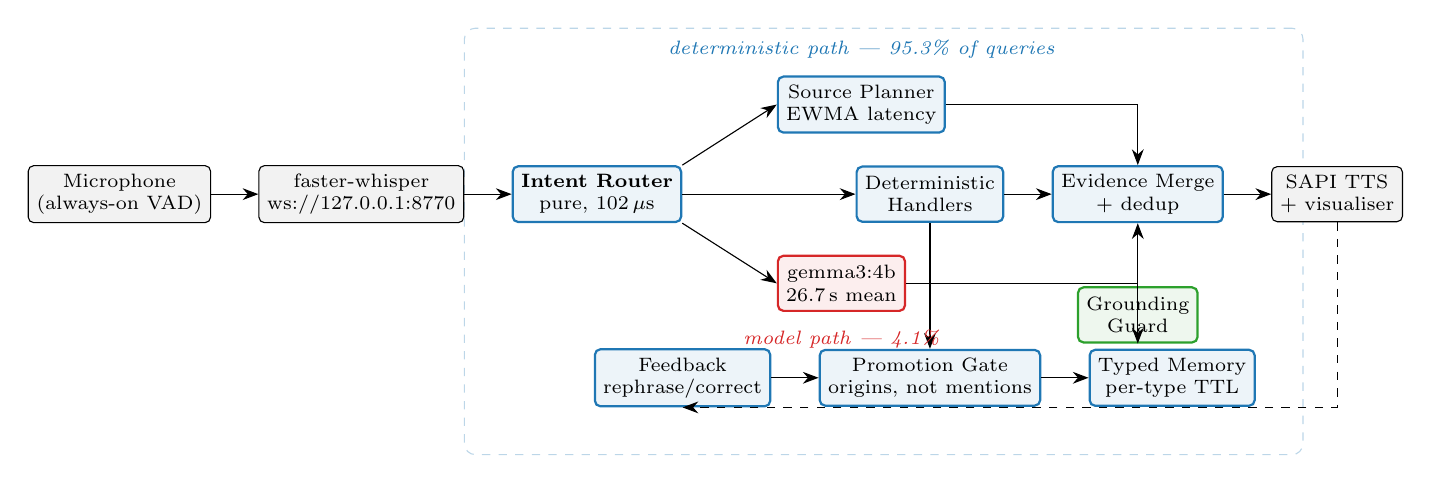
\begin{tikzpicture}[
  node distance=6mm,
  box/.style={draw, rounded corners=2pt, minimum height=7mm, align=center, font=\scriptsize, inner sep=3pt},
  detbox/.style={box, draw=det, fill=det!8, thick},
  modbox/.style={box, draw=mod, fill=mod!8, thick},
  verbox/.style={box, draw=ver, fill=ver!8, thick},
  ar/.style={-{Stealth[length=2mm]}, thin},
]

\node[box, fill=black!5] (mic) {Microphone\\(always-on VAD)};
\node[box, right=of mic, fill=black!5] (stt) {faster-whisper\\ws://127.0.0.1:8770};
\node[detbox, right=of stt] (router) {\textbf{Intent Router}\\pure, 102\,$\mu$s};

\node[detbox, above right=4mm and 12mm of router] (planner) {Source Planner\\EWMA latency};
\node[detbox, right=22mm of router] (handlers) {Deterministic\\Handlers};
\node[modbox, below right=4mm and 12mm of router] (model) {gemma3:4b\\26.7\,s mean};

\node[detbox, right=of handlers] (merge) {Evidence Merge\\+ dedup};
\node[verbox, below=8mm of merge] (guard) {Grounding\\Guard};

\node[box, right=of merge, fill=black!5] (tts) {SAPI TTS\\+ visualiser};

\node[detbox, below=16mm of handlers] (gate) {Promotion Gate\\origins, not mentions};
\node[detbox, right=of gate] (mem) {Typed Memory\\per-type TTL};
\node[detbox, left=of gate] (fb) {Feedback\\rephrase/correct};

\draw[ar] (mic) -- (stt);
\draw[ar] (stt) -- (router);
\draw[ar] (router) -- (handlers);
\draw[ar] (router.north east) -- (planner.west);
\draw[ar] (router.south east) -- (model.west);
\draw[ar] (planner.east) -| (merge.north);
\draw[ar] (handlers) -- (merge);
\draw[ar] (model.east) -| (guard.south);
\draw[ar] (guard) -- (merge);
\draw[ar] (merge) -- (tts);
\draw[ar] (handlers.south) -- (gate.north);
\draw[ar] (gate) -- (mem);
\draw[ar] (fb) -- (gate);
\draw[ar, dashed] (tts.south) |- (fb.south);

\begin{scope}[on background layer]
\node[fit=(router)(handlers)(planner)(merge)(gate)(mem)(fb), draw=det!30, dashed, rounded corners, inner sep=6mm] {};
\end{scope}

\node[font=\scriptsize\itshape, det, above=1mm of planner] {deterministic path --- 95.3\% of queries};
\node[font=\scriptsize\itshape, mod, below=1mm of model] {model path --- 4.1\%};

\end{tikzpicture}
\caption{System architecture. Blue components are deterministic and pure; the red
component is the language model; green is verification. The dashed region is
capability-invariant --- differences in behaviour arise from what a policy chooses to
consult, not from model sampling. Measured: routing 102\,$\mu$s/prompt, model turn
26.7\,s mean.}
\label{fig:arch}
\end{figure*}

Figure~\ref{fig:arch} shows the full pipeline. Three properties characterise it.

\paragraph{Purity at the boundaries.} The intent router, source planner, memory store,
promotion gate, and feedback analyser are all pure functions --- no network, no model, no
clock except where injected. This makes them exhaustively testable without mocking an
LLM, and it is why the system carries 1373 assertions across 34 suites.

\paragraph{The model never computes a number.} Every quantity spoken to the user
originates from a handler that read it. This is not a stylistic preference; it is a
response to two observed failures documented in \S\ref{sec:limits}.

\paragraph{Main/renderer split.} Electron's main process cannot import renderer ES
modules. Modules requiring main-process access (chain watchers, RPC hedging, metric
stores, provider discovery) are written as root-level CommonJS; renderer services are ES
modules under \code{src/js/services/}.

\subsection{Voice pipeline}

Speech capture runs continuously. An adaptive noise-floor voice-activity detector
(3$\times$ floor, 320\,ms preroll, 880\,ms $\to$ 1.44\,s hangover after observing
mid-thought truncation) gates a WebSocket stream of PCM16 chunks to a local
\code{faster-whisper} server. The server must be launched with Python's \code{-I} flag;
without it, user-site packages pollute \code{sys.path} and \code{onnxruntime} crashes
with an access violation.

The capture path is defended in depth because it fails silently. Bluetooth earbuds
switching between A2DP and HFP profiles tear down the capture device mid-TTS. Mitigations:
unbounded restart with 3--15\,s backoff, \code{track.onended} handling, a 5\,s watchdog
that force-restarts if no audio frames arrive within 15\,s, and STT-server respawn. A
device selector excludes virtual and loopback inputs --- Stereo Mix causes the assistant
to transcribe its own speech.

\subsection{Text-to-speech and self-echo}

TTS uses Windows SAPI. Because SAPI audio bypasses Chromium's acoustic echo canceller,
the microphone is gated while synthesis is active. This gate demonstrably leaks, so a
word-overlap guard (60\% overlap against a 20\,s window of spoken text) suppresses
self-transcription. Streaming TTS speaks each completed sentence during token
generation, reducing time-to-first-word from 5--10\,s to 1--2\,s.

%------------------------------------------------------------------
\section{The Deterministic Routing Layer}
\label{sec:routing}

\subsection{Design}

The router is a cascade of ordered regular-expression matchers over the normalised
transcript, returning a typed intent object. Ordering matters and is load-bearing: phone
intents are checked before desktop intents so ``open chrome on my phone'' does not open
Chrome on the PC; Wi-Fi connection intents precede the settings matcher so ``connect to
my Redmi'' reaches \code{netsh} rather than a settings deep link.

\subsection{Why a router and not a classifier}

An LLM-based intent classifier was measured at 3.0\,s per call on this hardware. A
multi-step agentic loop of 5--20 steps therefore costs 15--60\,s of silence before the
assistant speaks. Against this, the regex router costs 102\,$\mu$s --- roughly
$3\times10^4$ times cheaper --- and is deterministic, testable, and inspectable.

The tradeoff is generalisation. A classifier handles paraphrase; a regex does not. Our
response is empirical: the 1000-prompt harness (\S\ref{sec:eval}) measures exactly where
the regex cascade fails, and each failure becomes a pinned regression.

\subsection{Intent families}

\begin{table}[h]
\centering\small
\begin{tabular}{@{}ll@{}}
\toprule
\textbf{Family} & \textbf{Ground truth source} \\
\midrule
\code{PRICE\_QUERY} & Alpaca / Yahoo chart endpoint \\
\code{QUANT\_QUERY} & local computation over series \\
\code{CHAIN\_QUERY} & Alchemy RPC (verified chains) \\
\code{ISSUANCE} & ERC-20 Transfer log scan \\
\code{WHALE\_SCAN} & per-transaction aggregation \\
\code{NEWS\_QUERY} & RSS/Atom feed registry \\
\code{SECURITY\_ADVISORY} & NVD, CISA, Chrome releases \\
\code{PREDICTION\_MARKET} & Polymarket, Kalshi \\
\code{SYS\_OVERVIEW} & OS telemetry poller \\
\code{WIFI\_INFO} & \code{netsh} + \code{Get-NetIPConfiguration} \\
\code{PHONE\_TOOL} & companion app over LAN WebSocket \\
\code{READ\_SCREEN} & \code{gemma3:4b} vision \\
\code{SELF\_CRITIQUE} & interaction-log analysis \\
\code{AI\_COMMAND} & \emph{model fallback} \\
\bottomrule
\end{tabular}
\caption{Intent families and the source of ground truth for each. Only the last invokes
the language model for an answer.}
\end{table}

%------------------------------------------------------------------
\section{Retrieval}
\label{sec:rag}

\subsection{Hybrid architecture}

Retrieval fuses lexical BM25 with dense retrieval (\code{nomic-embed-text}, 768-dim) via
reciprocal rank fusion at $k=60$, plus pseudo-relevance feedback as a separate fusion
list at weight 0.5 so a poor feedback pool can dilute but not corrupt the original
ranking.

\subsection{The inverted index}

The original BM25 implementation re-tokenised the entire corpus on every query, inside a
nested loop --- measured at \textbf{94\,ms per query at 5000 chunks} on the renderer
thread. Replacing it with a persistent inverted index (term $\to$ \{df, postings\}),
incremental on ingest and rebuilt on load, gave a \textbf{230--320$\times$ speedup with
top-10 rankings bit-identical}.

The bit-identity check was not ceremonial. It surfaced a genuine determinism bug:
equal-scoring chunks are common, and map-insertion order ranked them differently between
runs. An explicit index tie-break was added to both the BM25 sort and the RRF sort, since
rank position --- not merely recall --- drives downstream faithfulness.

\subsection{Late sentence selection}

Rather than returning whole passages, sentences within top passages are scored by
IDF-weighted query overlap with a mild lead bias, and the top 10 retained. Measured on
real ingested text: \textbf{81\% context reduction} (11396 $\to$ 2192 characters across
four queries) with correct evidence at rank 1--3 and byte-identical output across
repeated calls. The system falls back to whole chunks when nothing matches lexically.

\subsection{Selective reranking}

LLM reranking is gated on ambiguity: it fires only when $(s_1 - s_2)/s_1 < 0.15$, i.e.\
when rank order is genuinely fragile. Measured: the gate fires on $\sim$50\% of queries,
costs $\sim$4.8\,s when it fires versus $\sim$90\,ms when it skips, and changed rank-1 on
4/4 firings. Because 5\,s of added silence is unacceptable on the voice path, reranking
is opt-in and disabled for speech input.

\paragraph{A negative result.} Ollama exposes no rerank endpoint. Cross-encoder
reranking, which a design note had ranked as the highest-priority improvement, is
\emph{not available} on this stack.

%------------------------------------------------------------------
\section{Live Data Layers}
\label{sec:data}

\subsection{Provider discovery, not assertion}

Chain provider availability is \emph{discovered} by probing each candidate endpoint and
comparing the returned chain ID against the expected value, rather than asserted from a
static table. A transient-versus-verdict retry distinguishes a genuine unavailability from
a network blip:

\begin{lstlisting}[language=JavaScript]
const isTransient = (r) =>
  /timeout|failed|ENOTFOUND|ECONN|socket|
   network|http 5\d\d|http 429/i.test(r||'');
let r = await probeSlug(slug, key, meta.id);
if (!r.ok && isTransient(r.reason)) {
  r = await probeSlug(slug, key, meta.id, 10000);
}
\end{lstlisting}

This was added after observing Ethereum dropped from the verified set by a single 6\,s
timeout. Live result: \emph{bsc, base, arbitrum, ethereum} verified in 375\,ms;
\emph{optimism, polygon} unavailable on this key.

\subsection{Whale detection}

Naive log scanning double-counts: a single arbitrage transaction touching three pools was
announced as a \$27M movement three times. The correction aggregates per transaction and
identifies net source and sink:

\begin{lstlisting}[language=JavaScript]
const pureSenders   = [...sent].filter(
  ([a]) => !received.has(a));
const pureReceivers = [...received].filter(
  ([a]) => !sent.has(a));
const source = pick(pureSenders) || pick(sent);
const sink   = pick(pureReceivers)|| pick(received);
const roundTrip = !pureSenders.length
               || !pureReceivers.length;
\end{lstlisting}

All token amounts are handled as \code{BigInt} throughout; float arithmetic on wei
silently loses precision.

\paragraph{A boundary held.} Exchange-label attribution (``this went to Binance'') was
requested repeatedly and declined each time: that mapping is not on-chain data, and
presenting a guessed label beside a verified amount would contaminate a verified answer
with an unverified one.

\subsection{Prediction markets}

Two defects found by probing before building:

\begin{enumerate}\itemsep1pt
\item Polymarket's \code{?title=} parameter does not filter --- a search for
``bitcoin'' returned NBA and NFL markets. Corrected to \code{/public-search?q=}.
\item Kalshi returns prices as dollar strings: \code{"0.0120"} means 1.2\%, not 1.2.
A planned division by 100 would have produced a 100$\times$ error.
\item Kalshi silently ignores \code{category=}. Corrected to the \code{/series}
catalogue with \code{series\_ticker=}.
\end{enumerate}

A binary market is detected structurally and probability read from the YES leg
explicitly, rather than from whichever outcome ranks highest --- an inversion that would
report 30\% as 70\%.

%------------------------------------------------------------------
\section{Typed, Revisable Memory}
\label{sec:memory}

\begin{figure}[t]
\centering
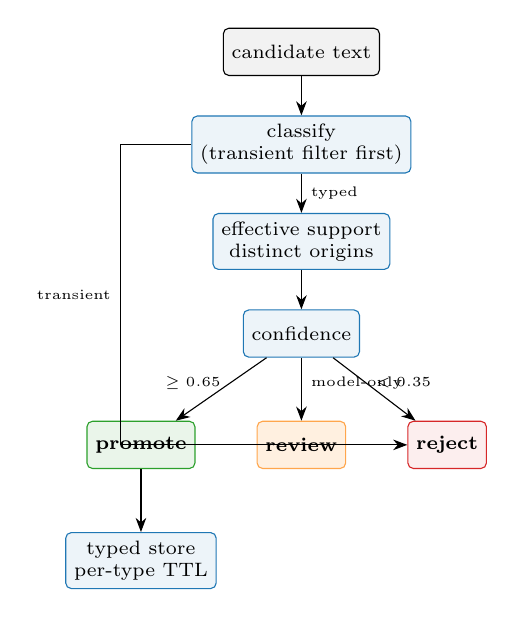
\begin{tikzpicture}[
  node distance=5mm,
  b/.style={draw, rounded corners=2pt, font=\scriptsize, align=center, minimum height=6mm, inner sep=3pt},
  ar/.style={-{Stealth[length=1.8mm]}, thin},
]
\node[b, fill=black!5] (cand) {candidate text};
\node[b, below=of cand, draw=det, fill=det!8] (cls) {classify\\(transient filter first)};
\node[b, below=of cls, draw=det, fill=det!8] (sup) {effective support\\distinct origins};
\node[b, below=of sup, draw=det, fill=det!8] (conf) {confidence};

\node[b, below left=8mm and 6mm of conf, draw=ver, fill=ver!10] (prom) {\textbf{promote}};
\node[b, below=8mm of conf, fill=orange!12, draw=orange!70] (rev) {\textbf{review}};
\node[b, below right=8mm and 6mm of conf, fill=mod!8, draw=mod] (rej) {\textbf{reject}};

\node[b, below=8mm of prom, draw=det, fill=det!8] (store) {typed store\\per-type TTL};

\draw[ar] (cand) -- (cls);
\draw[ar] (cls) -- node[right, font=\tiny] {typed} (sup);
\draw[ar] (sup) -- (conf);
\draw[ar] (conf) -- node[left, font=\tiny, pos=.4] {$\geq 0.65$} (prom);
\draw[ar] (conf) -- node[right, font=\tiny, pos=.4] {model-only} (rev);
\draw[ar] (conf) -- node[right, font=\tiny, pos=.4] {$< 0.35$} (rej);
\draw[ar] (prom) -- (store);
\draw[ar] (cls.west) -- ++(-9mm,0) |- node[left, font=\tiny, pos=.25] {transient} (rej.west);
\end{tikzpicture}
\caption{The promotion gate. Three outcomes, never two: a gate that can only accept or
drop pushes every uncertain case into one of the two failure modes.}
\label{fig:gate}
\end{figure}

\subsection{Why not a rolling summary}

The interaction log shows the same architectural questions re-asked days apart. A single
rolling summary is the wrong shape: it cannot be revised, so ``we use Etherscan'' and
``we replaced Etherscan'' both survive with no way to tell which holds.

Memory is instead a set of typed, individually revisable records. A revision replaces in
place, retains one hop of prior text, and counts itself.

\subsection{Retention is per type, not per age}

\begin{table}[h]
\centering\small
\begin{tabular}{@{}llc@{}}
\toprule
\textbf{Type} & \textbf{TTL} & \textbf{Revisable} \\
\midrule
\code{decision}    & never & yes \\
\code{constraint}  & never & yes \\
\code{preference}  & never & yes \\
\code{reference}   & never & yes \\
\code{bug}         & 180 d & yes \\
\code{benchmark}   & 90 d  & \textbf{no} \\
\code{experiment}  & 90 d  & no \\
\code{todo}        & 30 d  & yes \\
\bottomrule
\end{tabular}
\caption{Per-type retention. A decision made two years ago still governs the code; a
benchmark from two years ago is history.}
\end{table}

\paragraph{Benchmarks are deliberately non-revisable.} Overwriting 88.0\% with 99.4\%
destroys the series that makes either number meaningful. A new measurement is a new
record, and the write is rejected with a stated reason. This is verified end to end:
recording both leaves both in the store as a dated series.

\subsection{The promotion gate}

The central rule (Figure~\ref{fig:gate}) is that support is counted over \emph{distinct
origins}, not mentions:

\[
\text{eff}(\mathcal{O}) = \bigl|\{(o.\text{origin},\, o.\text{id}) : o \in \mathcal{O}\}\bigr|
\]

Origins are ranked \code{verified} $>$ \code{user} $=$ \code{handler} $>$ \code{model}.
Confidence derives from the strongest origin, nudged by corroboration from a
\emph{second independent} origin, and is capped below 1.0 --- nothing extracted from a
transcript is certain, and a stored 1.0 would read as verified when it is not.

\textbf{A model-only claim is never promoted outright}, whatever its score. This is the
specific path that produced the two fabrications documented in \S\ref{sec:limits}.

\subsection{Re-derivable answers are not memory}

Running the gate over the real 229-turn log revealed that \textbf{23 of 43 promotions
were stock quotes} --- ``Apple returned 55.2 percent annualized''. These carry numbers, so
they typed as benchmarks, but they are live-data \emph{answers}, stale within a day.
Storing one means retrieving a dead price later as durable project knowledge.

After correcting for this, telemetry did the same thing --- ``signal 100\%, 72.2
megabits'' promoted three times. The rule that emerged:

\begin{quote}\itshape
If a handler can fetch it again, it must fetch it again.
\end{quote}

Promotions fell from 43 to 17, then to 16 after a further word-order defect was found by
re-running the same benchmark.

%------------------------------------------------------------------
\section{Implicit Feedback}
\label{sec:feedback}

\subsection{Signals}

Three signals, none requiring the user to fill in a rating:

\begin{itemize}\itemsep1pt
\item \textbf{Rephrase}: near-repetition within 120\,s at token-overlap $\geq 0.6$
(asymmetric on the smaller set, since a rephrase is often shorter).
\item \textbf{Correction}: explicit lexical correction (``no'', ``that's wrong'',
``not what I meant'') following a prior turn.
\item \textbf{Fallback}: a factual question with a deterministic shape that reached
the model anyway.
\end{itemize}

\subsection{Struggles, not signals}

A run of rewordings on one subject is one problem, not $N$. Collapsing correlated signals
into \emph{resolution chains} prevents ranking a path by how stubborn the user was rather
than how wrong the path is. On the real log: \textbf{22 raw signals collapse to 18
struggles}, longest 3 turns, 16 of 18 resolved, 0 abandoned.

\subsection{Health normalised by usage}

\begin{table}[h]
\centering\small
\begin{tabular}{@{}lrrl@{}}
\toprule
\textbf{Path} & \textbf{per-100} & \textbf{turns} & \\
\midrule
\code{PHONE\_TOOL}  & 40.0 & 3   & worst \\
\code{QUANT\_QUERY} & 14.1 & 17  & \\
\code{AI\_COMMAND}  & 9.9  & 144 & healthiest per-turn \\
\bottomrule
\end{tabular}
\caption{Weighted failure per 100 turns on the real log. Raw counts would have named
\code{AI\_COMMAND} the problem; normalisation inverts the ordering.}
\end{table}

Weights: \code{corrected} 1.0 $>$ \code{fallback} 0.8 $>$ \code{rephrased} 0.6. A
correction is unambiguous; a rephrase may merely be a better wording.

\subsection{Gated to suggestions}

Signals become \code{confidence: 'review'} suggestions and stop. Two reasons: repeated
rephrases of a query may mean the \emph{symbol resolver} is thin rather than the routing
wrong; and the literature finds implicit feedback unreliable as a direct learning signal.
Nothing self-modifies.

\paragraph{An asymmetry to declare.} Observed feedback measures \emph{over-fetching}, not
\emph{under-fetching}. A source never consulted that would have helped is invisible.
Under-fetching surfaces instead as rephrases and corrections. Reading one without the
other makes an under-scoping planner look excellent.

%------------------------------------------------------------------
\section{Source Planning}
\label{sec:planner}

\begin{figure}[t]
\centering
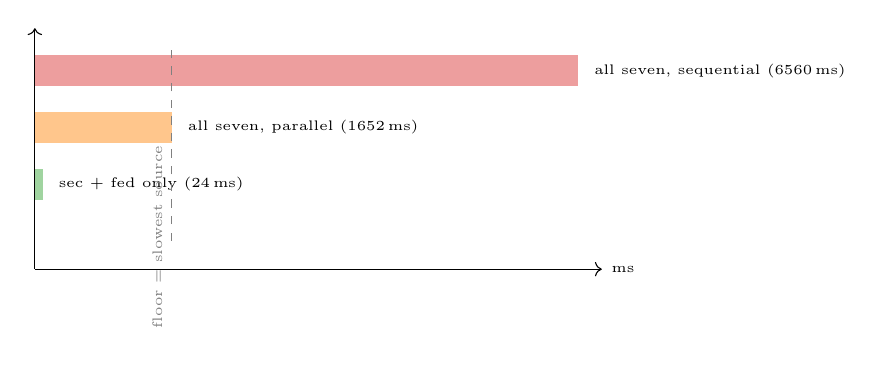
\begin{tikzpicture}[font=\scriptsize]
\begin{scope}[yscale=0.9]
\draw[->] (0,0) -- (7.2,0) node[right, font=\tiny] {ms};
\draw[->] (0,0) -- (0,3.4);

\foreach \y/\lbl/\w/\c in {
  2.8/{all seven, sequential (6560\,ms)}/6.9/mod,
  2.0/{all seven, parallel (1652\,ms)}/1.74/orange,
  1.2/{sec + fed only (24\,ms)}/0.10/ver}
  {\fill[\c!45] (0,\y-0.22) rectangle (\w,\y+0.22);
   \node[right, font=\tiny] at (\w+0.08,\y) {\lbl};}

\draw[dashed, gray] (1.74,0.4) -- (1.74,3.2);
\node[gray, font=\tiny, rotate=90, anchor=south] at (1.74,0.45)
  {floor = slowest source};
\end{scope}
\end{tikzpicture}
\caption{Measured feed retrieval. Parallel fan-out reaches the slowest single source
(chrome, 1650\,ms) within 2\,ms --- that is its floor. Selecting only the needed sources
is $\sim$69$\times$ better.}
\label{fig:planner}
\end{figure}

\subsection{The measurement that reframed the problem}

Seven live feeds, sequential: \textbf{6560\,ms}. In parallel: \textbf{1652\,ms}
(3.97$\times$). But the parallel total landed \emph{within 2\,ms of the slowest single
source} (chrome, 1650\,ms). That is the floor fan-out can reach. From the same run,
\code{sec-8k} measured 24\,ms and \code{fed} 18\,ms:

\[
\underbrace{1652\,\text{ms}}_{\text{all, parallel}}
\;\;\text{vs.}\;\;
\underbrace{24\,\text{ms}}_{\text{sec+fed only}}
\;\approx\; 69\times
\]

\textbf{The scheduler dominates the fan-out by roughly 17$\times$.} This is the opposite
of where the parallel-retrieval literature places its emphasis --- and the reason is
structural: those methods assume one homogeneous backend where every call costs the same.
These sources do not. \emph{Chrome is 92$\times$ slower than Fed.}

\subsection{Observed, not asserted}

Seed latencies from one run on one network would become exactly the kind of frozen
guess-map this project has a standing rule against. \code{observe()} replaces each seed
with an EWMA ($\alpha = 0.2$):

\[
\text{ms}_{t+1} = \alpha\,\text{ms}_{\text{obs}} + (1-\alpha)\,\text{ms}_t
\]

Verified: \code{fed} seeded at 18\,ms climbs to 751\,ms after eight slow responses, while
a single slow response moves it only to $\sim$194\,ms.

\paragraph{A failure carries no latency information.} It says the source was
\emph{unreachable}, not that it was slow. Failures therefore leave the latency estimate
untouched and lower reliability instead. Five chrome failures take reliability to 0.328
with latency unchanged. Folding a timeout into the latency average would make an
unreachable source merely look slow, and the planner would keep choosing it.

\subsection{Utility, not speed}

\[
u = \frac{\text{relevance} \times \text{reliability}}{\log_2\!\left(2 + \text{ms}/100\right)}
\]

A linear latency penalty drops chrome (1650\,ms) from Chrome-advisory queries entirely,
which is precisely wrong --- it is the \emph{only} source that can answer. The logarithmic
discount keeps a slow sole source in the plan while still preferring fast ones at equal
relevance.

\subsection{Merge and disclosure}

Merged results deduplicate by link-or-title and rank \emph{corroborated} items first:
appearance in two independent feeds is the only available evidence that a story is real
--- the same independence rule the promotion gate enforces, one layer up. A source that
fails to respond is disclosed aloud (``\ldots cisa did not respond, so this may be
incomplete''), because a missing source changes what the answer is allowed to claim.

%------------------------------------------------------------------
\section{Evaluation}
\label{sec:eval}

\subsection{The harness}

\code{eval/finance-prompts.mjs} generates 1000 prompts from catalogues already in the
repository --- 440 Ondo tokens from the user's own CSV, the six configured chains, the
verified feed domains. A prompt naming a ticker that does not exist tests only the error
path. Each prompt carries the intent it should reach, so the run scores routing
\emph{correctness}, not merely output.

\code{eval/agent-harness.mjs} runs a worker queue over the real router, with the router
context derived from the prototype so tests drive production code rather than a stub.

\subsection{Why routing at scale and the model by sample}

Sampling the real model path: mean \textbf{26{,}662\,ms}, p50 \textbf{30{,}444\,ms}, p95
\textbf{45{,}980\,ms} at concurrency 8. A thousand such turns projects to
\textbf{$\sim$56 minutes}. Routing all 1000 takes \textbf{103\,ms}.

That gap is the finding, not a workaround.

\subsection{Results}

\begin{table}[h]
\centering\small
\begin{tabular}{@{}lr@{}}
\toprule
\textbf{Metric} & \textbf{Value} \\
\midrule
Test suites / assertions & 34 / 1373 \\
Routing accuracy & 99.4\% (994/1000) \\
Routing cost & 103\,ms total, 102\,$\mu$s each \\
Answerable without model & \textbf{95.3\%} \\
Model-path share & 4.1\% \\
Model turn (mean / p95) & 26.7\,s / 46.0\,s \\
Feeds sequential $\to$ parallel & 6560 $\to$ 1652\,ms \\
Same benchmark, +2 days & 4248 $\to$ 938\,ms \\
BM25 index speedup & 230--320$\times$ \\
Late-selection context cut & 81\% \\
\bottomrule
\end{tabular}
\caption{Measured results. All figures from live runs on the author's machine.}
\end{table}

\subsection{Four defects the harness found}

Routing accuracy went \textbf{88.0\% $\to$ 99.4\%} after fixing four defects that
hand-written tests had not caught in months:

\begin{table}[h]
\centering\small
\begin{tabular}{@{}lp{3.4cm}@{}}
\toprule
\textbf{Prompt} & \textbf{Wrong behaviour} \\
\midrule
``what's happening with nvidia'' & returned CPU and RAM statistics (46 prompts) \\
``latest on ethereum'' & fell to the model (50 prompts) \\
``gas on bsc'' & fell to the model despite BSC being verified \\
``google stock price'' & \emph{typed} ``stock price'' into the focused window \\
\bottomrule
\end{tabular}
\end{table}

\subsection{The remaining six misses are deliberate}

``how much is intel'' is blocked by a known-symbol guard added after ``how much is
bitcoin'' produced a fabricated \$17{,}500. Loosening the guard to catch two more tickers
reopens that path. They are left visible rather than papered over.

\subsection{A defect in the harness itself}

One of the original five misses was ours: \code{HOT\_LIST} holds token records, not
strings, so the first run asked about ``tokenized [object Object]''. The harness scored it
as a miss --- which is the harness working.

%------------------------------------------------------------------
\section{Measurement Instability}
\label{sec:instab}

Re-running the feed benchmark two days later on \emph{identical code} returned 4248\,ms
sequential and 938\,ms parallel --- a 36\% shift, and a speedup of 4.53$\times$ rather
than 3.97$\times$.

This has a direct methodological consequence: \textbf{success criteria cannot be an
absolute latency number.} ``Achieves $<$1000\,ms'' would have passed on one day and failed
on the other, on code that never changed. Criteria must be a same-session A/B or a ratio.

It is also a live vindication of the EWMA decision: a frozen latency table written from
the first run would already have been 36\% wrong.

%------------------------------------------------------------------
\section{Limitations and Failures}
\label{sec:limits}

We report failures in the same detail as results.

\subsection{Two fabrications}

\begin{enumerate}\itemsep2pt
\item Asked for a CVE severity, the model produced \emph{CVE-2026-15905, ``Critical''}.
The correct rating was High. Corrected by the user, the model doubled down.
\item Asked ``how much is bitcoin'', the model produced \textbf{\$17,500} --- a number
from training data, presented as current.
\end{enumerate}

Both are one-shot generation with no observation step. The first fix attempted was a
guard blocking CVE identifiers; the user correctly objected that a guard only converts a
wrong answer into no answer. The real fix was integrating the actual advisory feeds.

\subsection{An untested retrieval layer}

\code{rag-store.json} contained \textbf{one chunk and zero vectors}. Every retrieval
improvement reported in \S\ref{sec:rag} is verified by harness, never by live usage. A
retrieval system with an empty corpus has a measurable \emph{implementation} and no
measurable \emph{quality}. Measuring the BM25 recall ceiling therefore has a precondition
that must be satisfied first.

\subsection{Voice transcription contaminates extraction}

Dictated speech reaches the constraint pattern through ``don't'': \emph{``i'll try to make
sure i don't get too deep''} is not a constraint, yet scores 0.7 on a single user origin.
This needs better candidate boundaries than one turn of speech. We decline to silence it
with a keyword blocklist, which would hide a segmentation problem rather than fix it.

\subsection{A feed echo}

A Chrome Releases feed headline was spoken aloud, transcribed back by the always-on
microphone, and routed as a user command to \code{PHONE\_TOOL}. Ingested text re-entering
the input path is an emergent interaction: every component behaved correctly in
isolation. It was found by \emph{reading the log for an unrelated reason}, and no metric
covers it.

\subsection{The unbuilt component}

The source planner decides what to fetch; \textbf{nothing yet executes the plan against
live feeds}. Until the fetch engine is wired, the measured 6560$\to$1652\,ms improvement
exists in a benchmark script and not in the user-facing path.

%------------------------------------------------------------------
\section{Methodology}
\label{sec:method}

\subsection{Probe before build}

Every endpoint is verified live before code depends on it. Four pasted specifications
were checked against reality and each contained an error that would otherwise have
shipped silently.

\subsection{Measure before optimise}

Three times in this work the measurement overturned the plan:

\begin{enumerate}\itemsep1pt
\item ``1000 chats'' became a worker queue, because a turn costs 26.7\,s.
\item 60\% of memory promotions were deleted, because they were stock quotes.
\item The scheduler beat the fan-out, because chrome is 92$\times$ slower than fed.
\end{enumerate}

None was predictable from the literature. Two \emph{contradicted} it.

\subsection{Anomaly $\to$ metric or test}

Every recurring anomaly becomes one or the other, and the choice depends on its shape:

\begin{table}[h]
\centering\small
\begin{tabular}{@{}ll@{}}
\toprule
\textbf{Question} & \textbf{Build} \\
\midrule
``How often does this happen?'' & metric \\
``Can this ever happen again?'' & regression test \\
\bottomrule
\end{tabular}
\end{table}

A rate deserves a meter; a correct value deserves a test. Metering everything produces
the appearance of observability while nobody reads the dashboard.

\subsection{Metrics confirm; browsing finds}

Instrumentation validates what is already suspected. The three most consequential
findings in this work --- the stock quotes in memory, the batch-size assumption in a cited
paper's own figure, and the feed echo --- all came from reading real data for a different
reason.

\subsection{Engineering knowledge is not uniform}

\begin{table}[h]
\centering\small
\begin{tabular}{@{}lll@{}}
\toprule
\textbf{Class} & \textbf{Enforceable} & \textbf{Example} \\
\midrule
Invariant & yes (test) & spoken output must never re-enter \\
Monitor & yes (metric) & source latency EWMA \\
Norm & no (review) & change begins with a hypothesis \\
\bottomrule
\end{tabular}
\end{table}

A constraint becomes operational only when something checks it. Until then it is a design
note with better formatting.

%------------------------------------------------------------------
\section{Discussion}

\subsection{What the architecture is actually optimising}

Not latency, and not cost. The measured 95.3\% figure is better read as a
\emph{robustness} result. The planning-language literature (\S\ref{sec:related}) shows
that as complexity grows, a model asked to produce the answer collapses while a model
asked to structure the problem degrades gracefully. Jarvis's deterministic handlers are
the extreme of that spectrum: for those queries the model produces neither the answer nor
the structure, and the failure mode disappears entirely.

\subsection{Where the system genuinely leads}

Not reasoning. On live local ground truth --- this machine's Wi-Fi quality, current gas on
Arbitrum, today's SEC filings, this phone's battery --- Jarvis answers from measurement
where a frontier model must search or guess. The defensible claim is narrow and true:
\emph{Jarvis answers from primary sources that general web search does not poll.}

\subsection{Where a small model still costs}

Everything in the remaining 4.1\%. Open-ended synthesis at 26.7\,s per turn is the
system's weakest surface, and no amount of routing removes it. The highest-leverage
remaining improvement is not a better prompt or a larger model but an
\emph{observation loop}: letting the model call a handler, see the actual result, and
revise. Both documented fabrications were one-shot generation with no observation step.
The constraint is the measured 3.0\,s per planning call, which bounds such a loop to 1--2
steps on the voice path.

%------------------------------------------------------------------
\section{Conclusion}

Jarvis demonstrates that a 4B-parameter local model can anchor a responsive voice
assistant provided the architecture stops treating it as the answer source. The measured
result --- 95.3\% of a realistic finance and blockchain prompt set answerable without the
model, at 102\,$\mu$s versus 26.7\,s --- is not primarily an efficiency claim. It is a
statement about where reliability comes from: from handlers that read reality, from gates
that count independent evidence rather than repetition, and from measurements taken
before rather than after the design is fixed.

The remaining work is stated plainly. The fetch engine is unbuilt, so the retrieval
speedup is not yet user-visible. The corpus is empty, so retrieval quality is unmeasured.
A feed echo remains unfixed. These are recorded here at the same resolution as the
results, because a system that reports only its successes has stopped being an instrument.

%------------------------------------------------------------------
\section*{Reproducibility}

\begin{lstlisting}[language=bash]
npm test                          # 34 suites, 1373 checks
node eval/agent-harness.mjs 1000  # routing, ~100ms
node eval/agent-harness.mjs 1000 --llm 25
node eval/record-benchmark.mjs --accuracy 99.4 --n 1000
\end{lstlisting}

Deterministic given the reported seed. Live-data figures depend on network conditions;
\S\ref{sec:instab} quantifies that dependence.

\section*{Acknowledgements}

Development was assisted by Claude Opus 4.8 (Anthropic) operating under a
measure-before-build discipline. Every quantitative claim in this paper corresponds to a
command that can be re-run.

\begin{thebibliography}{9}\small
\bibitem{formalizer} P.\ P.\ Kagitha et al.
  \emph{Unifying Inference-Time Planning Language Generation}. ACL 2026.
\bibitem{feedback} \emph{User Feedback in Human-LLM Dialogues: A Lens to Understand Users
  But Noisy as a Learning Signal}. arXiv:2507.23158.
\bibitem{promote} \emph{When Not to Write Memory: Governing False Promotion from
  Correlated Agent Traces}. arXiv:2607.02579.
\bibitem{cdic} \emph{Context-Driven Incremental Compression for Multi-Turn Dialogue
  Generation}. arXiv:2606.12411.
\bibitem{comem} Y.\ Zhang et al. \emph{CoMem: Context Management with A Decoupled
  Long-Context Model}. ICML 2026. arXiv:2605.30842.
\bibitem{compact} M.\ Cim et al. \emph{Parallel Context Compaction for Long-Horizon LLM
  Agent Serving}. arXiv:2605.23296.
\bibitem{ptet} Q.\ Su et al. \emph{Beyond Accuracy: Unveiling Inefficiency Patterns in
  Tool-Integrated Reasoning}. ACL 2026.
\bibitem{costbench} J.\ Liu et al. \emph{CostBench}. ACL 2026.
\bibitem{ranking} M.\ Hariri et al. \emph{Ranking Reasoning LLMs under Test-Time
  Scaling}. ACL 2026.
\bibitem{srgen} J.\ Mu et al. \emph{Self-Reflective Generation at Test Time}. ACL 2026.
\end{thebibliography}

\end{document}
